\documentclass{article}
\usepackage[utf8]{inputenc}
\usepackage{tikz}

\title{path-independence}
\author{ }
\date{January 2020}

\begin{document}

\maketitle

\section{Introduction}

Many systems can be understood as a a category, or a collection of sets, with some transformation functions between the sets- for example, in programming languages, type systems with coercion. If a graph is constructed with the sets as nodes and functions as edges between the nodes, then by construction the new graph has the property of "path independence", the idea being that each object has a unique representation in a given set in the system.

\section{Definitions}
\begin{enumerate}
    \item Path graph: A graph with vertices representing sets, and directed edges representing transformations functions between the sets. A path represents the composition of the transformation functions in the nodes.
    \item Conflicting paths: Paths with same source and destination node.
    \item Path independence: The property that all conflicting paths in a graph are equal. Equality can be thought of as evaluated by some function equality checking oracle.
\end{enumerate}

\section{Identifying the set of new conflictiong paths on addition of edge}
\subsection{Theorem 1: The result of the two-flip tolerant path search algorithm corresponds bijectively to the set of new conflicting paths that arise in the graph dues to the addition of an edge.}

Proof:\\
Let the new edge added to the graph be (s,t).
The two flip tolerant path algorithm returns all paths from s to t with upto two direction flips.

*This proof is straightforward*

\subsection{Implementation of two-flip tolerant path search}
Normal recursive DFS with visited set also getting popped on backtrack (to get \textit{all} paths) but with direction and number of flips parameters to maintain state.

\subsection{Verification using the new paths}
The appropriate function and function inverse compositions.

\subsubsection{If any of the paths don't check out then the graph cannot be path independent. If all the paths do check out and the graph was originally path independent then the new graph is path independent.}

\subsection{Theorem: If the two flip tolerant path search returns two paths P and Q that have the same flipping points then they provide the same information and one can be removed as redundant}

\begin{center}
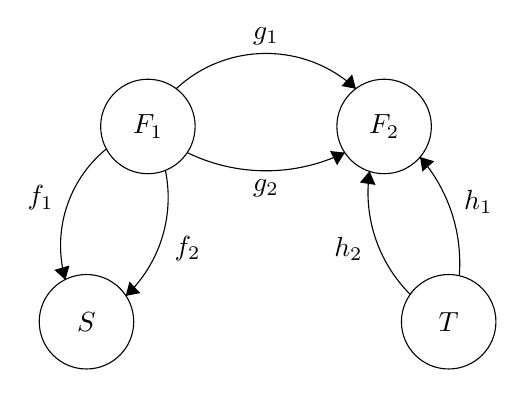
\begin{tikzpicture}[scale=0.2]
\tikzstyle{every node}+=[inner sep=0pt]
\draw [black] (25,-31.9) circle (3);
\draw (25,-31.9) node {$S$};
\draw [black] (48,-31.9) circle (3);
\draw (48,-31.9) node {$T$};
\draw [black] (28.9,-19.5) circle (3);
\draw (28.9,-19.5) node {$F_1$};
\draw [black] (43.9,-19.5) circle (3);
\draw (43.9,-19.5) node {$F_2$};
\draw [black] (30.687,-17.11) arc (132.96162:47.03838:8.383);
\fill [black] (42.11,-17.11) -- (41.87,-16.2) -- (41.19,-16.93);
\draw (36.4,-14.36) node [above] {$g_1$};
\draw [black] (41.409,-21.156) arc (-63.93383:-116.06617:11.399);
\fill [black] (41.41,-21.16) -- (40.47,-21.06) -- (40.91,-21.96);
\draw (36.4,-22.82) node [below] {$g_2$};
\draw [black] (23.657,-29.237) arc (-164.08097:-230.83744:7.929);
\fill [black] (23.66,-29.24) -- (23.92,-28.33) -- (22.96,-28.61);
\draw (22.95,-24.04) node [left] {$f_1$};
\draw [black] (30.007,-22.272) arc (11.75211:-46.67052:8.58);
\fill [black] (27.49,-30.26) -- (28.42,-30.08) -- (27.73,-29.35);
\draw (30.56,-27.24) node [right] {$f_2$};
\draw [black] (45.566,-30.169) arc (-134.8387:-188.56886:9.123);
\fill [black] (42.98,-22.34) -- (42.36,-23.06) -- (43.35,-23.21);
\draw (42.57,-27.26) node [left] {$h_2$};
\draw [black] (46.175,-21.439) arc (41.169:-4.57656:10.227);
\fill [black] (46.18,-21.44) -- (46.33,-22.37) -- (47.08,-21.71);
\draw (48.95,-24.27) node [right] {$h_1$};
\end{tikzpicture}
\end{center}

Intuitive sketch:
Let path $P_1$ be $f_1\circ g_1 \circ h_1$. Let path $P_2$ be $f_2\circ g_2 \circ h_2$. Then the equality constraint checking leads to identical results.

\subsubsection{Theorem: If two paths have one flip-point in common and there exist some path connecting the second flip points, then there exists a partial ordering between the two paths}

Two possible cases:


\begin{center}
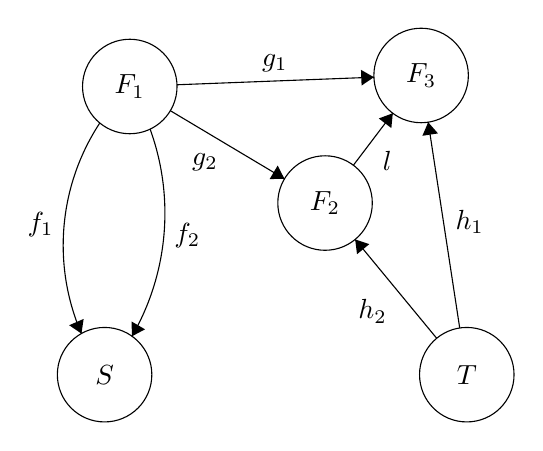
\begin{tikzpicture}[scale=0.2]
\tikzstyle{every node}+=[inner sep=0pt]
\draw [black] (25,-31.9) circle (3);
\draw (25,-31.9) node {$S$};
\draw [black] (48,-31.9) circle (3);
\draw (48,-31.9) node {$T$};
\draw [black] (26.6,-13.6) circle (3);
\draw (26.6,-13.6) node {$F_1$};
\draw [black] (39,-21) circle (3);
\draw (39,-21) node {$F_2$};
\draw [black] (45.1,-12.9) circle (3);
\draw (45.1,-12.9) node {$F_3$};
\draw [black] (29.18,-15.14) -- (36.42,-19.46);
\fill [black] (36.42,-19.46) -- (35.99,-18.62) -- (35.48,-19.48);
\draw (31.38,-17.8) node [below] {$g_2$};
\draw [black] (23.529,-29.292) arc (-156.64712:-213.3464:14.141);
\fill [black] (23.53,-29.29) -- (23.67,-28.36) -- (22.75,-28.76);
\draw (21.8,-22.39) node [left] {$f_1$};
\draw [black] (27.889,-16.304) arc (19.98764:-29.98116:15.634);
\fill [black] (26.74,-29.46) -- (27.57,-29.02) -- (26.71,-28.52);
\draw (29.4,-23.08) node [right] {$f_2$};
\draw [black] (46.09,-29.59) -- (40.91,-23.31);
\fill [black] (40.91,-23.31) -- (41.03,-24.25) -- (41.81,-23.61);
\draw (42.95,-27.88) node [left] {$h_2$};
\draw [black] (29.6,-13.49) -- (42.1,-13.01);
\fill [black] (42.1,-13.01) -- (41.28,-12.54) -- (41.32,-13.54);
\draw (35.81,-12.7) node [above] {$g_1$};
\draw [black] (47.55,-28.93) -- (45.55,-15.87);
\fill [black] (45.55,-15.87) -- (45.18,-16.73) -- (46.17,-16.58);
\draw (47.25,-22.21) node [right] {$h_1$};
\draw [black] (40.8,-18.6) -- (43.3,-15.3);
\fill [black] (43.3,-15.3) -- (42.41,-15.63) -- (43.21,-16.24);
\draw (42.63,-18.35) node [right] {$l$};
\end{tikzpicture}
\end{center}

$P_2$ is better, intuitively because l can only lose- not add information.


\begin{center}
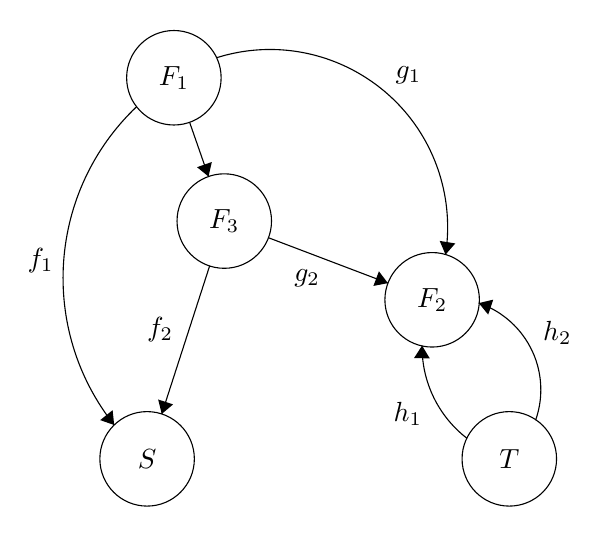
\begin{tikzpicture}[scale=0.2]
\tikzstyle{every node}+=[inner sep=0pt]
\draw [black] (25,-31.9) circle (3);
\draw (25,-31.9) node {$S$};
\draw [black] (48,-31.9) circle (3);
\draw (48,-31.9) node {$T$};
\draw [black] (26.7,-7.7) circle (3);
\draw (26.7,-7.7) node {$F_1$};
\draw [black] (43.1,-21.8) circle (3);
\draw (43.1,-21.8) node {$F_2$};
\draw [black] (29.9,-16.8) circle (3);
\draw (29.9,-16.8) node {$F_3$};
\draw [black] (29.408,-6.43) arc (107.51449:-8.88948:11.282);
\fill [black] (43.95,-18.93) -- (44.57,-18.22) -- (43.58,-18.06);
\draw (41.59,-8.14) node [above] {$g_1$};
\draw [black] (22.914,-29.751) arc (-141.57162:-226.46499:15.013);
\fill [black] (22.91,-29.75) -- (22.81,-28.81) -- (22.02,-29.44);
\draw (19.1,-19.32) node [left] {$f_1$};
\draw [black] (46.06,-22.008) arc (71.20036:-19.43982:5.814);
\fill [black] (46.06,-22.01) -- (46.66,-22.74) -- (46.98,-21.79);
\draw (50.12,-23.9) node [right] {$h_2$};
\draw [black] (45.319,-30.601) arc (-127.57654:-180.66292:7.327);
\fill [black] (42.46,-24.71) -- (41.95,-25.5) -- (42.95,-25.52);
\draw (42.49,-29.07) node [left] {$h_1$};
\draw [black] (28.97,-19.65) -- (25.93,-29.05);
\fill [black] (25.93,-29.05) -- (26.65,-28.44) -- (25.7,-28.13);
\draw (26.68,-23.67) node [left] {$f_2$};
\draw [black] (32.71,-17.86) -- (40.29,-20.74);
\fill [black] (40.29,-20.74) -- (39.72,-19.99) -- (39.37,-20.92);
\draw (35.16,-19.83) node [below] {$g_2$};
\draw [black] (27.7,-10.53) -- (28.9,-13.97);
\fill [black] (28.9,-13.97) -- (29.11,-13.05) -- (28.17,-13.38);
\end{tikzpicture}
\end{center}

$P_1$ is better for a similar reason.

\subsubsection{Theorem: In general, if there is an ordering to be derived from a paths between both flipping points of two paths, then there might exists a partial ordering between the two paths}

I think the only case we know for sure is this one:


\begin{center}
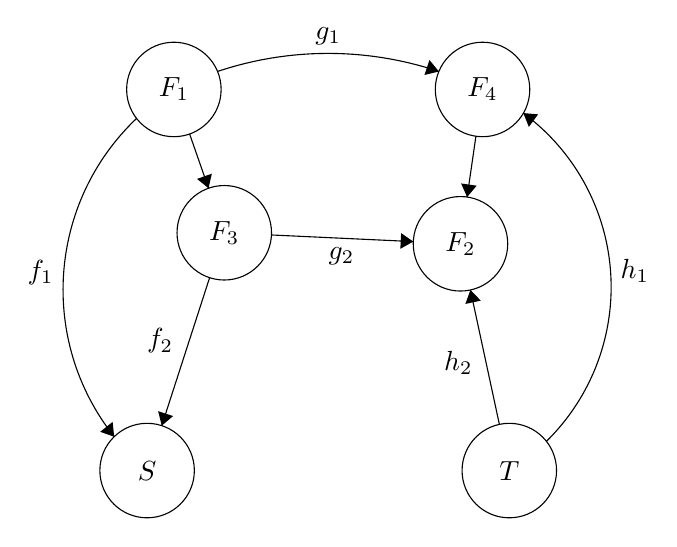
\begin{tikzpicture}[scale=0.2]
\tikzstyle{every node}+=[inner sep=0pt]
\draw [black] (25,-31.9) circle (3);
\draw (25,-31.9) node {$S$};
\draw [black] (48,-31.9) circle (3);
\draw (48,-31.9) node {$T$};
\draw [black] (26.7,-7.7) circle (3);
\draw (26.7,-7.7) node {$F_1$};
\draw [black] (44.9,-17.5) circle (3);
\draw (44.9,-17.5) node {$F_2$};
\draw [black] (29.9,-16.8) circle (3);
\draw (29.9,-16.8) node {$F_3$};
\draw [black] (46.3,-7.7) circle (3);
\draw (46.3,-7.7) node {$F_4$};
\draw [black] (22.914,-29.751) arc (-141.57162:-226.46499:15.013);
\fill [black] (22.91,-29.75) -- (22.81,-28.81) -- (22.02,-29.44);
\draw (19.1,-19.32) node [left] {$f_1$};
\draw [black] (47.37,-28.97) -- (45.53,-20.43);
\fill [black] (45.53,-20.43) -- (45.21,-21.32) -- (46.19,-21.11);
\draw (45.7,-25.06) node [left] {$h_2$};
\draw [black] (28.97,-19.65) -- (25.93,-29.05);
\fill [black] (25.93,-29.05) -- (26.65,-28.44) -- (25.7,-28.13);
\draw (26.68,-23.67) node [left] {$f_2$};
\draw [black] (32.9,-16.94) -- (41.9,-17.36);
\fill [black] (41.9,-17.36) -- (41.13,-16.82) -- (41.08,-17.82);
\draw (37.34,-17.71) node [below] {$g_2$};
\draw [black] (27.7,-10.53) -- (28.9,-13.97);
\fill [black] (28.9,-13.97) -- (29.11,-13.05) -- (28.17,-13.38);
\draw [black] (29.471,-6.557) arc (108.53192:71.46808:22.115);
\fill [black] (43.53,-6.56) -- (42.93,-5.83) -- (42.61,-6.78);
\draw (36.5,-4.91) node [above] {$g_1$};
\draw [black] (45.88,-10.67) -- (45.32,-14.53);
\fill [black] (45.32,-14.53) -- (45.93,-13.81) -- (44.94,-13.67);
\draw [black] (48.889,-9.204) arc (53.58054:-45.54392:13.727);
\fill [black] (48.89,-9.2) -- (49.24,-10.08) -- (49.83,-9.28);
\draw (55.03,-19.24) node [right] {$h_1$};
\end{tikzpicture}
\end{center}
I think $P_1$ is better. Don't yet have a proof sketch in mind yet but this is what the intuition from the previous cases would lead to.

The two other cases arise when you flip each arrow in turn. I think in these cases the result might go either way; TODO come up with the appropriate counterexamples.

\section{Optimized Algorithm}
Here, present pseudocode to do the path search with the ignoring of useless possibilities baked in. Perform runtime analysis.

\end{document}
